\documentclass[11pt]{article}
\usepackage[margin=0.9in]{geometry}
\usepackage{booktabs,array}
\usepackage{amsmath}
\usepackage{graphicx}
\usepackage[font=small,labelfont=bf]{caption}
\usepackage{enumitem}
\usepackage{xcolor}
\usepackage{hyperref}

\setlength{\parskip}{0.35em}
\setlength{\parindent}{0em}

\title{\Large\textbf{IRC Results Snapshot}\\[4pt]
\normalsize Refined GAD $\rightarrow$ IRC validation, status as of 2026-04-15}
\author{}
\date{}

\begin{document}
\begin{center}\fbox{\parbox{0.95\textwidth}{\small\textbf{SUPERSEDED 2026-04-20.} First-pass IRC validation snapshot. Current canonical: \texttt{IRC\_COMPREHENSIVE\_2026-04-20.pdf}. Kept for record.}}\end{center}
\vskip0.5em
\maketitle
\thispagestyle{empty}

\section*{What This Note Covers}

This note summarizes the \emph{current} IRC validation workflow and the latest
scientifically meaningful refined rerun. It is intentionally compact: the goal is
to preserve the key numbers, the threshold analysis, and a small amount of
interpretation in one place.

\textbf{Pipeline used here}
\begin{enumerate}[nosep,leftmargin=1.5em]
\item Start from converged GAD trajectories from \texttt{noise\_survey\_300}.
\item These trajectories come from \textbf{dataset TS geometries} with Gaussian noise added
      to the \texttt{Transition1x} labeled transition-state coordinates.
\item Select a TS candidate from the saved trajectory (\texttt{best\_nneg1}).
\item Recompute projected TS quality with HIP:
      $n_{\text{neg}}$, force norm, and $f_{\max}$.
\item If needed, refine the TS candidate with projected GAD.
\item Run IRC \emph{from that TS} in both downhill directions using Sella's IRC routine.
\item Compare the two endpoints against the \texttt{Transition1x} labeled reactant/product
      using:
      aligned geometry (element-aware Kabsch/Hungarian RMSD) and bond-topology matching.
\end{enumerate}

\textbf{Important interpretation point}
The current labels \texttt{intended / half / unintended} mean:
\emph{does the HIP IRC from this GAD-found TS recover the dataset-labeled
reactant/product pair?} This is a strong benchmark, but not a complete
unsupervised analysis of all possible connected minima on HIP's PES.

\section*{Run Summary}

The refined rerun analyzed here is the completed array \texttt{59385481\_[0-2]}.
It covered 30 converged TS candidates each at noise levels 0, 10, and 50 pm.

\begin{center}
\begin{tabular}{lrrrrrr}
\toprule
Noise & Total & IRC ran & Criterion failed & Intended & Half & Topology-half only / Unintended \\
\midrule
0 pm  & 30 & 15 & 15 & 1 & 3 & 1 / 10 \\
10 pm & 30 &  7 & 23 & 0 & 2 & 1 / 4 \\
50 pm & 30 &  3 & 27 & 0 & 0 & 1 / 2 \\
\bottomrule
\end{tabular}
\end{center}

\textbf{Headline:} the dominant failure mode is now \texttt{ts\_quality\_gate\_failed},
not code failure. The looser refined criterion did recover one fully intended case at
0 pm and increased IRC attempts there (15 instead of 12), but the attempted cases
still become progressively worse with noise: a few mixed / half-intended outcomes
at low noise and mostly unintended behavior by 50 pm.

\section*{Main Figure}

\begin{center}
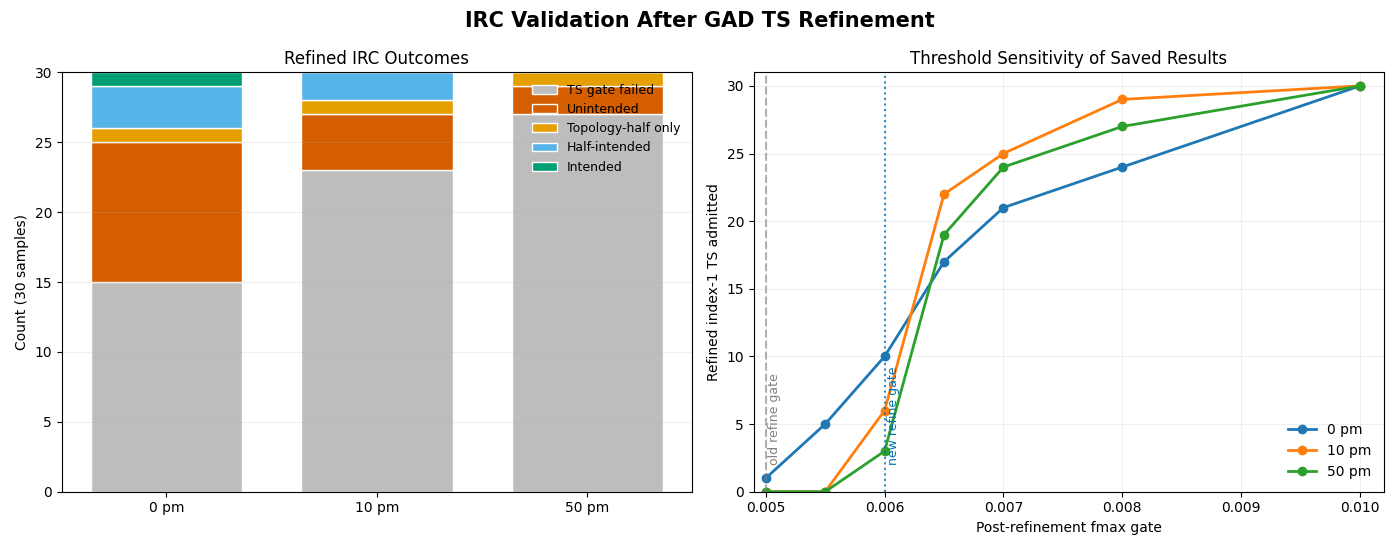
\includegraphics[width=\textwidth]{figures/fig_irc_refined_summary.png}
\captionof{figure}{\textbf{Left:} outcome breakdown of the refined rerun.
\textbf{Right:} number of refined index-1 candidates that would pass under looser
post-refinement $f_{\max}$ criteria, using the already-saved results.}
\end{center}

\textbf{Interpretation}
\begin{itemize}[nosep,leftmargin=1.5em]
\item Noise hurts in two layers:
      fewer candidates survive TS screening, and the surviving ones connect less
      cleanly to the labeled endpoints.
\item Even 0 pm is only partially ``clean'' under the stricter pipeline: one
      intended case, a few half-intended cases, and many criterion failures. This means
      the old convergence notion (\(n_{\text{neg}}=1\) plus loose force screening)
      was broad enough that some nominally converged points were not clean TSs by
      stricter \(f_{\max}\)-based standards.
\item The threshold-sweep panel shows why moving from \(f_{\max}<0.005\) to
      \(f_{\max}<0.006\) was justified. The current rerun already reflects that
      change.
\end{itemize}

\section*{Why The Force Criterion Was Too Strict}

\begin{center}
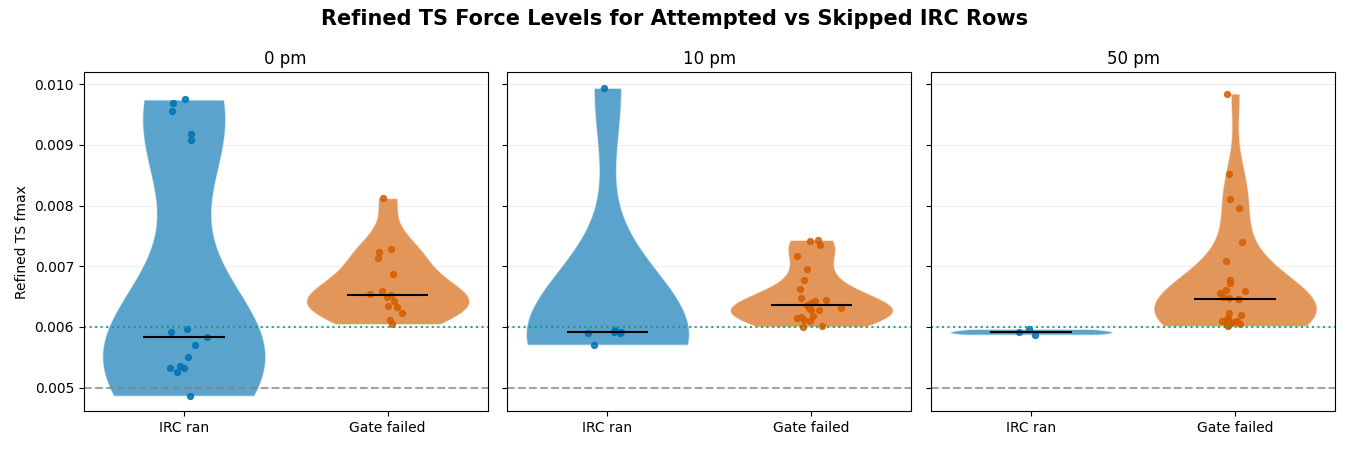
\includegraphics[width=\textwidth]{figures/fig_irc_refined_fmax.png}
\captionof{figure}{Refined TS \(f_{\max}\) for rows that actually ran IRC versus rows
that were skipped by the TS-quality criterion. Dashed gray: old refined criterion \(0.005\).
Dotted green: new refined criterion \(0.006\).}
\end{center}

\textbf{Most important observation:}
the previous policy had been asymmetric, and the current rerun is the first one
after correcting that.

\begin{itemize}[nosep,leftmargin=1.5em]
\item Unrefined candidates could go straight to IRC if they satisfied
      \(f_{\max}<0.01\).
\item Refined candidates were only allowed through if they satisfied
      \(f_{\max}<0.005\).
\end{itemize}

That old policy meant some \emph{improved} refined TSs were being rejected even
though their \(f_{\max}\) was smaller than already-accepted unrefined TSs. The
current rerun used the corrected post-refinement criterion \(f_{\max}<0.006\).

\begin{center}
\begin{tabular}{lrrr}
\toprule
Noise & Max accepted pre-criterion \(f_{\max}\) & Min rejected refined \(f_{\max}\) & Median rejected refined \(f_{\max}\) \\
\midrule
0 pm  & 0.009748 & 0.006202 & 0.006533 \\
10 pm & 0.009941 & 0.006007 & 0.006357 \\
50 pm & ---      & 0.006018 & 0.006456 \\
\bottomrule
\end{tabular}
\end{center}

\textbf{Conclusion:}
\begin{itemize}[nosep,leftmargin=1.5em]
\item \(0.005\) was stricter than necessary for a first refined IRC pass.
\item The current rerun confirms that \(f_{\max}<0.006\) is a reasonable next
      operating point: it increases attempted IRC at 0 pm and recovers one intended
      case without simply reverting to the original \(0.01\) screen.
\item The remaining failed-criterion rows are now clustered around
      \(0.0062\text{--}0.0065\), which is tighter and more interpretable than the
      old \(0.0052\text{--}0.0059\) bottleneck.
\end{itemize}

\section*{Updated Rerun Settings}

The new defaults already patched into the repo are:

\begin{itemize}[nosep,leftmargin=1.5em]
\item \texttt{--refine-steps 600} instead of 300
\item \texttt{--refine-force-threshold 0.006} instead of 0.005
\end{itemize}

Why 600 steps? In the completed refined rerun, the refinement stage still
occasionally hit the new 600-step cap, especially at 50 pm:
\begin{center}
\begin{tabular}{lrr}
\toprule
Noise & Rows hitting 600-step refinement cap & Mean refinement steps \\
\midrule
0 pm  &  2 & 87 \\
10 pm &  0 & 127 \\
50 pm &  3 & 201 \\
\bottomrule
\end{tabular}
\end{center}

So the main gain from the latest rerun came from the looser refined criterion rather
than dramatically longer refinement trajectories; most cases did not use the full
600-step budget.

\section*{What To Inspect First In 3D}

The viewer bundles from the completed refined run are already available under:
\texttt{/lustre07/scratch/memoozd/gadplus/runs/irc\_validation\_300/viewer\_noise\_*pm/viewer\_bundle/}

Recommended cases:
\begin{itemize}[nosep,leftmargin=1.5em]
\item \texttt{0 pm / sample 31}: the one fully intended case in the latest rerun
\item \texttt{0 pm / samples 0, 33, 45}: representative low-noise half-intended cases
\item \texttt{10 pm / samples 51, 175}: useful geometry-vs-topology disagreement cases
\item \texttt{50 pm / sample 175}: topology-half at high noise
\item \texttt{50 pm / samples 20, 89}: clearly unintended high-noise examples
\end{itemize}

Each bundle contains:
\begin{itemize}[nosep,leftmargin=1.5em]
\item dataset reactant reference
\item reverse IRC endpoint
\item TS input
\item forward IRC endpoint
\item dataset product reference
\end{itemize}

So this is an endpoint/context view of the IRC outcome, not a dense movie of every
internal IRC integration step.

\section*{Bottom Line}

\begin{itemize}[nosep,leftmargin=1.5em]
\item The current refined IRC pipeline is now producing \emph{real} scientific signal.
\item The main issue is TS admissibility, not numerical IRC crashes.
\item Noise degrades both TS quality and endpoint agreement.
\item The latest rerun under \(f_{\max}<0.006\) is better at 0 pm, but high-noise
      cases remain dominated by criterion failures and unintended endpoints.
\item The next decision point is not ``whether to loosen from 0.005'' anymore;
      that is already done. The next question is whether further loosening or a
      different TS-selection/refinement strategy is justified.
\end{itemize}

\section*{What Is Running Right Now}

\textbf{Queue snapshot captured at 2026-04-15 17:22 UTC}

\begin{center}
\begin{tabular}{>{\ttfamily}l>{\ttfamily}lcc>{\ttfamily}l}
\toprule
JobID & Name & State & Time & Node / Reason \\
\midrule
59385266\_1 & run\_nr\_then\_gad.slur & R & 1:17:47 & ng20601 \\
59385266\_2 & run\_nr\_then\_gad.slur & R & 1:17:47 & ng20601 \\
59385266\_3 & run\_nr\_then\_gad.slur & R & 1:17:47 & ng30102 \\
59385266\_4 & run\_nr\_then\_gad.slur & R & 1:17:47 & ng30102 \\
59385266\_5 & run\_nr\_then\_gad.slur & R & 1:17:47 & ng30102 \\
59385266\_7 & run\_nr\_then\_gad.slur & R & 1:17:47 & ng20401 \\
59385266\_8 & run\_nr\_then\_gad.slur & R & 1:17:47 & ng20401 \\
59385266\_9 & run\_nr\_then\_gad.slur & R & 1:17:47 & ng20401 \\
59385266\_10 & run\_nr\_then\_gad.slur & R & 1:14:18 & ng30104 \\
59385266\_11 & run\_nr\_then\_gad.slur & R & 1:14:18 & ng20401 \\
\bottomrule
\end{tabular}
\end{center}

The latest IRC rerun \texttt{59385481\_[0-2]} has already completed. The jobs
still running now are the \texttt{run\_nr\_then\_gad} experiments shown above.

\end{document}
